% Rapport final, projet A2 (GAN sur MNIST, générateur fixe).
% Compiler : python tools/build.py   (pdflatex deux fois -> report.pdf ; pages PNG : python tools/render.py <dossier>)
% Chaque partie vit dans sections/<partie>.tex ; les figures dans figures/, tracées par figscripts/<partie>.py.
\documentclass[10pt,twocolumn]{article}
% Préambule : article deux colonnes, aéré et lisible : Times 10 pt, interligne légèrement ouvert,
% gouttière large, paragraphes séparés par un petit blanc, légendes courtes.
% Encadré \takeaway{...} : la phrase à retenir d'une partie. \tabnote{...} : note sous un tableau.
\usepackage[T1]{fontenc}
\usepackage[utf8]{inputenc}
\usepackage{amsmath}
\usepackage{mathptmx}
\usepackage[a4paper,margin=1.9cm,columnsep=0.75cm]{geometry}
\usepackage{microtype}
\usepackage{graphicx}
\usepackage{booktabs}
\usepackage{tabularx}
\usepackage{xcolor}
\usepackage[font=small,labelfont=bf,labelsep=period,skip=5pt]{caption}
\captionsetup[table]{position=top,skip=4pt}
\usepackage{enumitem}
\usepackage{titlesec}
\usepackage[numbers,sort&compress]{natbib}
\usepackage[hidelinks]{hyperref}
\graphicspath{{figures/}}
\linespread{1.06}
\setlength{\parindent}{0pt}
\setlength{\parskip}{4.5pt plus 1pt}
\setlist{itemsep=2pt,topsep=2pt,leftmargin=1.2em}
\titleformat{\section}{\normalfont\large\bfseries}{\thesection}{0.6em}{}
\titleformat{\subsection}{\normalfont\normalsize\bfseries}{\thesubsection}{0.5em}{}
\titlespacing*{\section}{0pt}{12pt plus 3pt}{4pt}
\titlespacing*{\subsection}{0pt}{8pt plus 2pt}{2pt}
\setlength{\textfloatsep}{12pt plus 3pt}
\setlength{\floatsep}{10pt plus 2pt}
\setlength{\dbltextfloatsep}{12pt plus 3pt}
\setlength{\intextsep}{10pt plus 2pt}
\renewcommand{\topfraction}{0.8}
\renewcommand{\dbltopfraction}{0.8}
\renewcommand{\textfraction}{0.15}
\renewcommand{\floatpagefraction}{0.75}
\renewcommand{\arraystretch}{1.12}
\definecolor{accent}{HTML}{1F6FC5}
\definecolor{muted}{HTML}{52514E}
\newcommand{\takeaway}[1]{\par\smallskip\noindent\colorbox{accent!7}{\parbox{\dimexpr\linewidth-2\fboxsep}{\textbf{In short.} #1}}\par\smallskip}
\newcommand{\tabnote}[1]{\par\vspace{3pt}{\footnotesize #1\par}}
\newcommand{\finc}{FID$_\text{Inc}$}
\newcommand{\fcnn}{FID$_\text{CNN}$}

\raggedbottom % pas d'étirement vertical entre paragraphes en bas de colonne
\titlespacing*{\paragraph}{0pt}{4pt plus 1pt}{0.6em} % \paragraph aussi serré que les sous-sections

\begin{document}

% ---------- Page de garde (hors des 5 pages de contenu) : titre, résumé, figure de synthèse ----------
\onecolumn
\thispagestyle{empty}
\begin{center}
\vspace*{1.2cm}
{\LARGE\bfseries Improving a fixed-architecture GAN on MNIST:\\[4pt] what helps, why, and when it fails\par}
\vspace{0.6cm}
{\large Quentin Revillon \quad Noé Mosca \quad Nicodème Gorge\par}
\vspace{0.2cm}
{Group 3 --- DataLab, Master IASD \quad {\color{muted}November 2026}\par}
\vspace{0.5cm}{\color{muted}\rule{0.8\textwidth}{0.4pt}}\vspace{0.4cm}

\begin{minipage}{0.8\textwidth}
\small\textbf{Abstract.}
The generator of our GAN on MNIST is a fixed MLP. We change one lever at a time (data, training, inference)
under a common protocol (3 seeds, 10\,000 samples, MNIST test) and rank models with the Inception FID
(FID$_\text{Inc}$), as the course platform does.
\textbf{Training gives the gain, but only as a pair:} a relativistic loss with R1 alone leaves FID$_\text{Inc}$
flat (38.7\,$\to$\,37.7) while it fixes the digit mix; EMA alone gives 30.0; together,
\textbf{38.7\,$\pm$\,1.2\,$\to$\,22.1\,$\pm$\,1.3} (submitted model: platform FID \textbf{21.59}).
\textbf{Data levers do not help:} instance selection costs recall; instance noise neither lowers FID$_\text{Inc}$
nor prevents collapses.
\textbf{Rejection sampling needs a discriminating $D$:} on the final model it helps only once $D$ is
recalibrated (OBRS, \textbf{22.0\,$\to$\,19.7}, 33\% acceptance).
A FID in the features of our MNIST classifier tracks the digit mix, which weighs about ten times less in
FID$_\text{Inc}$.
\end{minipage}

\vspace{0.8cm}
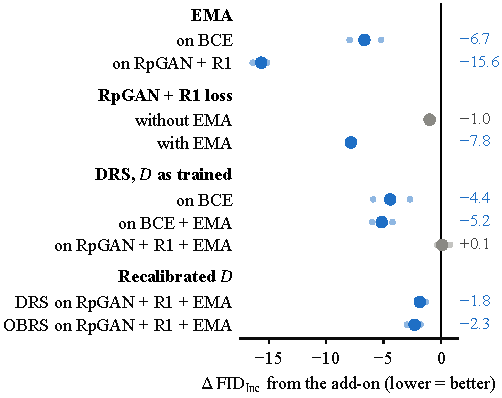
\includegraphics[width=0.62\textwidth]{combination_effects}
\captionsetup{width=0.8\textwidth}
\captionof{figure}{\textbf{Gain of each add-on, by base model} ($\Delta$FID$_\text{Inc}$, lower is better).
Large dot: mean; small dots: seeds (paired runs). Blue: $p<0.05$ (paired $t$-test; Welch for the loss rows,
unpaired). Rows on the RpGAN $G_\text{EMA}$ and samplers on BCE: cluster re-sampling, 2 draws per seed.}
\label{fig:combination-effects}
\end{center}
\clearpage
\setcounter{page}{1}

% Partie intro : le problème en mots simples, le protocole, le tableau de synthèse des leviers.
% Sources : PLAN.md §0-§5 ; results/comparison_local.csv (baseline Mac) ; enquete/results/juliet/juliet2_test.csv
% (BCE brut / EMA, cluster) ; drs_recalib_test.csv (rejet) ; nico_data_test.csv (levier données) ; puissance : PLAN.md l. 215.
\section{Introduction}\label{sec:intro}

A generative adversarial network (GAN) is made of two neural networks trained against each other. The
\emph{generator} $G$ turns a vector of random numbers $z$ into an image; the \emph{discriminator} $D$ receives real and
generated images and learns to tell them apart. $G$ improves by fooling $D$, and $D$ improves by not being fooled. Once
training is over, only $G$ is kept: each new $z$ gives a new handwritten digit.

In this project the architecture of $G$ is imposed: a small fully connected network that maps 100 random numbers to
$28\times28$ pixels. We cannot make it bigger or smarter, so we work on the three things that remain:
\begin{itemize}
\item the \textbf{data} it learns from (Sec.~\ref{sec:data});
\item the \textbf{training} procedure: loss function and discriminator (Sec.~\ref{sec:training});
\item the \textbf{inference}, i.e.\ how images are drawn once $G$ is trained (Sec.~\ref{sec:inference}).
\end{itemize}

\textbf{How we compare methods.} A GAN trained twice with different random seeds gives different results, so a single
run proves little. Every variant is therefore trained with three seeds under the same conditions: the same 50\,000
training images (10\,000 more are kept aside for validation), the same budget of 200 epochs, and the last checkpoint is
used. Each trained model draws 10\,000 images, which are compared with the 10\,000 images of the MNIST test set. We report
the mean and standard deviation over seeds, and use $t$-tests to decide whether a difference is real. With three seeds,
only differences of about 3.6 points of FID are reliably detectable; smaller ones may exist but stay hidden in the noise
between seeds.

The score is the one of the course platform: the \textbf{Fréchet Inception Distance} (\finc{}, lower is better), which
measures how far generated images are from real ones in the eyes of a pretrained image network. Sec.~\ref{sec:fid} explains
why we chose it over a variant built on a digit classifier. Two companion scores read the trade-off: \textbf{precision}
(the share of generated images that look like real ones: quality) and \textbf{recall} (the share of real images that the
generator can imitate: diversity)~\cite{kynkaanniemi2019}.

\textbf{Baseline.} The provided code (standard GAN loss, no extra trick) reaches \finc{} $38.7\pm1.2$, precision 0.47 and
recall 0.51. Fig.~\ref{fig:samples}a shows its samples: readable digits, but many ``1''s and ``7''s and few ``2''s.

Table~\ref{tab:summary} summarizes what each lever brought. The rest of the report follows the same plan for each method:
what it does, what the literature led us to expect, what we observed, and why.

\begin{table}[t]
\centering\small
\setlength{\tabcolsep}{3pt}
\caption{\textbf{What each lever brought.} \finc{} before $\to$ after the change (lower is better), mean of 3 seeds or more.}
\label{tab:summary}
\begin{tabular}{@{}llrl@{}}
\toprule
Lever & Change & \finc{} & Verdict \\
\midrule
Data      & keep 90\% most typical images & $35.4\to35.8$ & no gain \\
          & keep 50\% most typical images & $35.4\to47.8$ & worse \\
          & noise on $D$'s inputs         & $30.0\to30.1$ & no gain \\
\midrule
Training  & average $G$'s weights (EMA)   & $36.6\to30.0$ & \textbf{better} \\
          & + relativistic loss and R1    & $30.0\to22.1$ & \textbf{better} \\
\midrule
Inference & filter images with $D$        & $22.0\to22.1$ & no gain \\
          & same, $D$ recalibrated        & $22.0\to19.7$ & \textbf{better} \\
\bottomrule
\end{tabular}
\tabnote{Data rows: separate protocol with its own reference (Sec.~\ref{sec:data}). Inference rows: on the final model.}
\end{table}

\begin{figure*}[t]
\centering
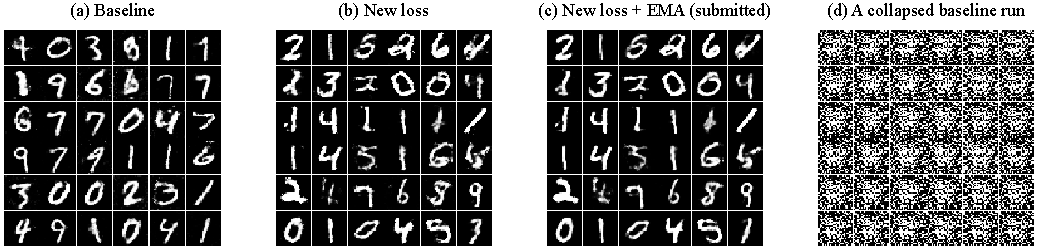
\includegraphics[width=\textwidth]{combination_samples}
\caption{\textbf{Samples from the same 36 random vectors $z$.} (a) Baseline: readable, but many ``1''s and ``7''s.
(b) New loss (Sec.~\ref{sec:training}): all digits appear. (c) Same run with averaged weights: cleaner strokes; this is the
submitted model. (d) A baseline run that collapsed: $G$ only outputs noise.}
\label{fig:samples}
\end{figure*}

% Partie fid : quelle mesure mène, et pourquoi un FID CNN à côté du FID Inception.
% Sources : PLAN.md §2, §5.1 ; enquete/fid.md ; baseline.md §3 ; enquete/results/juliet/{sensitivity_10k,kid_perclass_all}.csv ;
% enquete/results/fid/{rank_correlation,variance_share}.csv ; results/comparison_local.csv (sd entre seeds, ddof = 1).
% Plancher par chiffre : 8,5 (kid_perclass_all.csv 8,547) ; PLAN.md écrit 8,6 par erreur d'arrondi.
% Figure : figscripts/fid.py.
\section{Which FID? Evaluation}\label{sec:fid}

We add FID$_\text{CNN}$: in-domain (a LeNet replaces Inception on MNIST in~\cite{binkowski2018}), seconds instead of ${\approx}40$\,min of CPU (so tracked every epoch), and meant to see missing digits, the typical failure of an unconditional GAN.
The two FIDs can rank models oppositely: which should lead?

\paragraph{Measures.}
For features $\phi$ of real ($r$) and generated ($g$) images, with means $\mu$ and covariances $\Sigma$~\cite{heusel2017},
\[
\mathrm{FID}=\lVert\mu_r-\mu_g\rVert^2+\mathrm{Tr}\bigl(\Sigma_r+\Sigma_g-2(\Sigma_r\Sigma_g)^{1/2}\bigr).
\]
\textbf{FID$_\text{Inc}$}: $\phi$ = 2048-d pool layer of Inception-v3 (ImageNet).
\textbf{FID$_\text{CNN}$}: $\phi$ = 128-d penultimate layer of our MNIST classifier (98.7\% test accuracy).
\textbf{KID}: unbiased squared MMD, Inception features~\cite{binkowski2018}.
\textbf{P}: share of generated images inside the $k$-NN radius ($k{=}5$) of a real image, VGG features; \textbf{R}: real and generated swapped~\cite{kynkaanniemi2019}.
\textbf{Floor} (finite-$N$ bias~\cite{chong2020}): MNIST train vs test, 1.53 (Inc), 2.74 (CNN).

\paragraph{Expected.}
A FID follows the classes of its network~\cite{kynkaanniemi2023}: ImageNet has no digit class, our CNN has ten, so FID$_\text{CNN}$ should see the digit mix, FID$_\text{Inc}$ the appearance~\cite{heusel2017}.
Yet Lucic et al.\ find FID$_\text{Inc}$ on MNIST ``heavily influenced by the missing modes''~\cite{lucic2018}.

\begin{figure}[t]
\centering
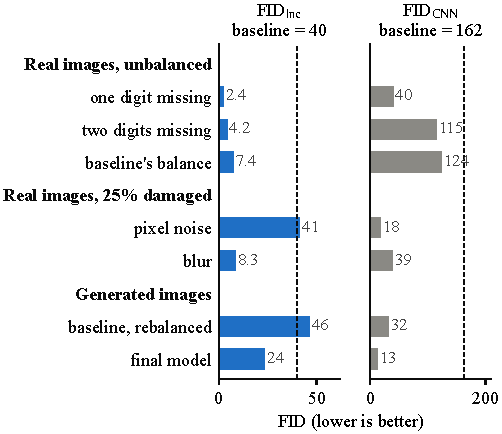
\includegraphics[width=\columnwidth]{fid_sensitivity}
\caption{\textbf{How much each FID sees each defect.} Each defect is added to real images; bar = its FID as a share of the baseline's gap to real data, $(\mathrm{FID}-\text{floor})/(\mathrm{FID}_\text{base}-\text{floor})$. $\mathrm{FID}_\text{base}$: baseline seed~0 (39.9 Inc, 162 CNN). Digit mix: 3 draws; other rows: one.}
\label{fig:fid-sensitivity}
\end{figure}

\paragraph{Observed.}
\begin{itemize}
\item \textbf{Dosed defects} (Fig.~\ref{fig:fid-sensitivity}): FID$_\text{Inc}$ weighs the digit mix about ten times less than FID$_\text{CNN}$, pixel noise ten times more; blur, blends and erasing weigh alike. Digit identity explains 67\% of the CNN feature variance, 26\% of Inception's.
\item \textbf{Rebalancing} baseline samples to the test digit mix: FID$_\text{CNN}$ 162\,$\to$\,32, but FID$_\text{Inc}$ \emph{rises} 39.9\,$\to$\,46.2 (badly drawn rare digits enter).
\item \textbf{Checkpoint:} FID$_\text{CNN}$ picks epoch 106, FID$_\text{Inc}$ epoch 200 ($\rho{=}{-}0.885$ after epoch 100): the digit imbalance grows while FID$_\text{Inc}$ falls.
\item \textbf{Seeds:} relative sd 11--25\% (FID$_\text{CNN}$) vs 3--6\% (FID$_\text{Inc}$), from the mix, not estimator noise (floor sd 0.19).
\item \textbf{KID} agrees with FID$_\text{Inc}$ (Spearman 0.96) and, like it, does not separate the baseline from raw RpGAN + R1 ($p=0.16$).
\end{itemize}

\paragraph{Per-digit FID$_\text{Inc}$.}
The CNN labels 100\,000 samples; 1\,000 per digit are scored against the test images of that digit; we average the ten (floor 8.5).
No frequency weighting: the baseline's ``2'' scores 113 (real 10.2) but makes up 1.6\% of images, so the global FID barely sees it (Sec.~\ref{sec:training}).
Limit: the CNN forces every image into a digit (confidence ${<}\,0.9$: 12.6\% of baseline images, 3.7\% of real ones).

\paragraph{When each measure fails.}
\begin{itemize}
\item \textbf{FID$_\text{CNN}$:} circular for instance selection (same features, Sec.~\ref{sec:data}); classifier-dependent (142--224 on the same images, three CNN seeds); saturating (final model: 6\% of the baseline gap vs 57\% in FID$_\text{Inc}$; on 6 RpGAN generators the FIDs disagree, $\rho{=}0.14$); it chose our $\gamma$ (Sec.~\ref{sec:training}); not comparable to papers or the platform.
\item \textbf{FID$_\text{Inc}$, P/R:} agree weakly with humans; DINOv2 is recommended~\cite{stein2023} (untested; we inspect samples, as the platform does).
\end{itemize}

\begin{table}[t]
\centering\footnotesize
\caption{\textbf{Which measure answers which question.}}
\label{tab:fid-roles}
\begin{tabular}{@{}ll@{}}
\toprule
Question & Measure \\
\midrule
Rank models, final scores & FID$_\text{Inc}$ + P/R (VGG, $k{=}5$) \\
Stroke quality at fixed digit & mean per-digit FID$_\text{Inc}$ \\
Digit mix & digit histogram (FID$_\text{CNN}$ as diagnostic) \\
Comparison with papers & FID$_\text{Inc}$ only \\
\bottomrule
\end{tabular}
\end{table}

\takeaway{FID$_\text{CNN}$ mostly measures the digit mix, FID$_\text{Inc}$ the appearance, and FID$_\text{Inc}$ even rewards dropping hard digits: use each measure for its own question (Table~\ref{tab:fid-roles}).}

% Part "data": instance selection and instance noise (Nicodeme's lever).
% Numbers: enquete/results/juliet/nico_data_test.csv (data runs), juliet2_test.csv (BCE+EMA +- noise, Juliet),
% results/comparison_local.csv (BCE and RpGAN + R1 + EMA +- noise, Mac), enquete/data.md (mechanics, collapse counts, DeVries).
% Paired rerun 9/11 (noise_03_e100 vs data_ref_e100, seeds 0-7, 60k updates): enquete/results/juliet/noise_rerun_test.csv.
% Figure: figscripts/data.py -> figures/data_selection_pr.pdf.
\section{Data: instance selection and instance noise}
\label{sec:data}

\textbf{Setup.} Data protocol (Table~\ref{tab:intro-protocol}), raw $G$. Compare FIDs only within a block of Table~\ref{tab:data-results}.

\begin{table}[t]
\centering\footnotesize
\setlength{\tabcolsep}{4pt}
\caption{\textbf{Data lever.} FID$_\text{Inc}$ (mean $\pm$ sd) and P/R (VGG), healthy runs.}
\label{tab:data-results}
\begin{tabular}{@{}lrrrr@{}}
\toprule
Variant & Coll. & FID$_\text{Inc}$ & P & R \\
\midrule
\multicolumn{5}{@{}l}{\emph{Data runs: BCE, no EMA, 120k updates (cluster)}} \\
Reference          & 3/8\rlap{$^a$} & 35.4\,$\pm$\,0.9 & 0.51 & 0.52 \\
Selection 95\%     & 2/5 & 38.2\,$\pm$\,2.7 & 0.49 & 0.48 \\
Selection 90\%     & 2/5 & 35.8\,$\pm$\,3.3 & 0.53 & 0.49 \\
Selection 75\%     & 0/3 & 40.8\,$\pm$\,3.9 & 0.54 & 0.40 \\
Selection 50\%     & 4/8 & 47.8\,$\pm$\,2.9 & 0.56 & 0.32 \\
Noise $\sigma_0{=}0.1$ & 4/8 & 35.5\,$\pm$\,2.5 & 0.52 & 0.52 \\
Noise $\sigma_0{=}0.3$ & 0/3 & 37.0\,$\pm$\,1.6 & 0.51 & 0.52 \\
\midrule
\multicolumn{5}{@{}l}{\emph{Paired rerun: same, 60k updates, seeds 0--7 (cluster)}} \\
Reference          & 3/8 & 55.3\,$\pm$\,2.6 & 0.29 & 0.42 \\
Noise $\sigma_0{=}0.3$ & 1/8 & 54.3\,$\pm$\,3.9 & 0.29 & 0.40 \\
\midrule
\multicolumn{5}{@{}l}{\emph{Common protocol (50k split, 200 epochs), $G_{\mathrm{EMA}}$}} \\
BCE + EMA (cluster)        & 0/3\rlap{$^b$} & 30.0\,$\pm$\,0.2 & 0.56 & 0.54 \\
\quad + noise 0.3         & 2/5 & 30.1\,$\pm$\,1.3 & 0.56 & 0.54 \\
RpGAN + R1 + EMA (Mac)    & 0/3 & 22.1\,$\pm$\,1.3 & 0.59 & 0.59 \\
\quad + noise 0.3         & 0/3 & 21.4\,$\pm$\,0.6 & 0.60 & 0.61 \\
\bottomrule
\end{tabular}
\tabnote{Coll.: collapsed runs (R $<0.01$) / seeds. $^a$0/3 on seeds 0--2 (those of noise 0.3). $^b$0/6 with 3 Mac runs. Mac vs cluster: ${\approx}\,2$ FID.}
\end{table}

\subsection{Instance selection}
\textbf{Method.} Score each training image $x$ of digit $c$ by $s(x) = -(f(x)-\mu_c)^\top \Sigma_c^{-1} (f(x)-\mu_c)$; $f$: 128-d feature of the FID$_\text{CNN}$ network (trained on the same 60k images); $\mu_c, \Sigma_c$: its per-digit mean and covariance. Keep the top 95, 90, 75 or 50\% of each digit.

\textbf{Expected.} Keeping the most typical half of ImageNet: FID 21.4 $\to$ 12.6, P $+0.11$, R $-0.03$~\cite{devries2020}, but with a conditional SAGAN (64$\times$64, halved capacity) and FID in the selection's own space.

\textbf{Observed} (Welch vs reference). No rate wins: 90\% ties ($p = 0.83$), 95\% and 75\% are worse within noise ($p = 0.19$, $0.13$), 50\% is clearly worse ($p = 0.002$). At 50\%, R falls in both feature spaces (VGG $-0.20$, $p < 10^{-6}$; CNN $-0.37$; Fig.~\ref{fig:data-selection-pr}): circularity amplifies the loss, it does not create it. P rises significantly only in the selection CNN; in VGG ($p = 0.22$) it partly reflects easier digits (``1'': 28\% $\to$ 35\% of samples).

\begin{figure}[t]
\centering
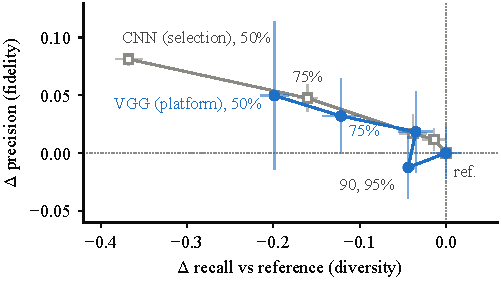
\includegraphics[width=\columnwidth]{data_selection_pr}
\caption{\textbf{Selection costs recall in both feature spaces;} precision gains only in the selection CNN. Change vs the 100\% reference; labels: share kept; bars: sd.}
\label{fig:data-selection-pr}
\end{figure}

\textbf{Why.} (i) The training set stays balanced, yet the unconditional $G$ drops whole digits (``0'': 10.2\% $\to$ 0.0\% at 50\%). (ii) MNIST's tail is likely diversity, not errors: 50\% selection of the \emph{real} images cuts their CNN recall from 0.89 to 0.63. (iii) Capacity is likely not the bottleneck: the same $G$ reaches 22.1 (Sec.~\ref{sec:training}).

\textbf{When it fails.} Already in the paper at 256$\times$256 (BigGAN, 9.8 $\to$ 10.6). Without its random-50\% control (22.8), we cannot separate ``fewer'' from ``chosen'' images.

\subsection{Instance noise}
\textbf{Method.} $D$ sees $x + \sigma_t \varepsilon$, $\varepsilon \sim \mathcal{N}(0, I)$, real and fake (pixels in $[-1,1]$); $\sigma_t$ decays from $\sigma_0$ to 0 at epoch 101 of 200, so FIDs measure only a lasting effect.

\textbf{Expected.} Overlap keeps $D$ imperfect and $G$'s gradient alive~\cite{arjovsky2017,sonderby2017}: stability, no FID gain.

\textbf{Observed.} No significant FID$_\text{Inc}$ effect (Table~\ref{tab:data-results}; Welch $p \ge 0.21$). On raw $G$, noise worsens BCE ($36.6 \to 42.5$, $p = 0.03$; n.s.\ after Bonferroni). No detectable effect on collapses: 2/5 vs 0/6 with EMA (Fisher $p = 0.18$); in the paired 8-seed rerun, 1/8 with noise vs 3/8 without ($p = 0.57$), healthy FID 54.3 vs 55.3 ($p = 0.58$). The earlier ``0 of 8'' with noise does not replicate.

\textbf{Why.} \emph{Collapses are numerical:} all 19 collapsed data runs end with a vanishing gradient for $G$; in 17, $D(G(z)) < 10^{-12}$, where \texttt{BCELoss} clamps its denominator, so the gradient decays as $e^{\text{logit}}$. \emph{Noise does not stop $D$:} one direction separates real from fake, while noise spreads over all pixels~\cite{roth2017}; against the initial $G$, $D$ still reaches 100\% accuracy for $\sigma \le 1$. \emph{With RpGAN}, R1 already is deterministic instance noise~\cite{roth2017,mescheder2018}.

\textbf{When it fails.} Noise ($\sigma_0 \le 0.3$) does not replace a numerically safe loss: \texttt{BCEWithLogitsLoss} keeps the gradient at 1; RpGAN + R1 never collapsed (0/6).

\takeaway{On clean MNIST with an unconditional $G$, data levers do not lower FID$_\text{Inc}$: selection costs recall; noise neither helps nor prevents collapses, which are numerical (sigmoid + \texttt{BCELoss}).}

% Partie training (Noé Mosca) : perte relativiste, R1 et EMA.
% Chiffres : enquete/results/juliet/juliet2_test.csv (BCE brut / EMA, A100), results/comparison_local.csv (baseline Mac, RpGAN + EMA),
% enquete/results/ema/ema_summary.csv (RpGAN brut), kid_perclass_all.csv (FID par chiffre), enquete/training.md (balayage gamma,
% effondrements, équilibre de D), PLAN.md §2 (réplication A100). Figure : figscripts/training.py -> figures/training_perdigit.pdf.
\section{Training: relativistic loss, R1 and EMA}\label{sec:training}

\textbf{Hypotheses.} H1: the sigmoid BCE saturates (collapse) and drifts to easy digits; a relativistic loss with R1 keeps $G$'s gradient informative. H2: averaging $G$'s weights removes the oscillation around equilibrium.

\textbf{Method.} $D(x)$: raw score of $D$ (before the sigmoid); $\mathrm{sp}(t)=\log(1+e^t)$. RpGAN~\cite{jolicoeur2019} scores a pair (real $x$, fake $\tilde x$); R1~\cite{mescheder2018} penalises $D$'s slope on real images (we omit R2, its fake-image twin in R3GAN~\cite{huang2024}):
\begin{align*}
L_D &= \mathrm{sp}\big(D(\tilde x)-D(x)\big) + \tfrac{\gamma}{2}\,\|\nabla_x D(x)\|^2,\\
L_G &= \mathrm{sp}\big(D(x)-D(\tilde x)\big).
\end{align*}
EMA~\cite{yazici2019}: after each step, $G_\mathrm{EMA}\leftarrow\beta\,G_\mathrm{EMA}+(1-\beta)\,G$, $\beta=0.999$ (half-life $\approx$\,1.4 epochs). Training uses only raw $G$: each run yields both, so EMA effects are paired.

\begin{figure}[t]
\centering
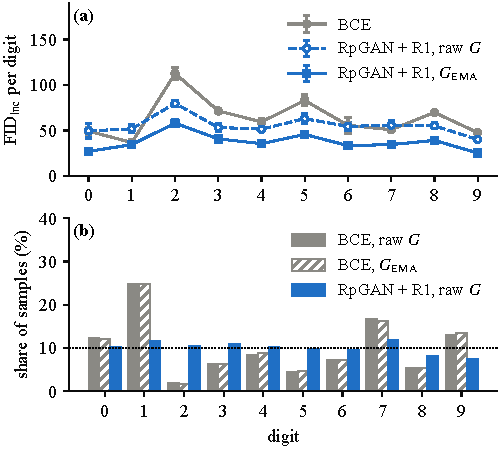
\includegraphics[width=\columnwidth]{training_perdigit}
\caption{\textbf{RpGAN + R1 fixes the digit mix; EMA cleans every digit.} Common protocol, 3 seeds. (a) Per-digit FID$_\text{Inc}$ (real data: 6.5--10.4). (b) Share of each digit in 10\,000 samples (dotted: 10\%). BCE: Mac in (a), cluster in (b).}
\label{fig:training-perdigit}
\end{figure}

\begin{table}[t]
\centering\footnotesize\setlength{\tabcolsep}{3pt}
\caption{\textbf{Loss $\times$ EMA} (common protocol).}
\label{tab:training-ema}
\begin{tabular}{@{}llcccc@{}}
\toprule
 & & \multicolumn{2}{c}{BCE} & RpGAN + R1 & Loss $\Delta$\\
\cmidrule(lr){3-4}
 & & Mac & cluster & Mac & ($p$)\\
\midrule
raw $G$ & FID$_\text{Inc}$ & 38.7$\pm$1.2 & 36.6$\pm$1.3 & 37.7$\pm$1.0 & $-1.0$ (0.35)\\
 & P/R & 0.47/0.51 & 0.48/0.49 & 0.47/0.47 & \\
$G_\mathrm{EMA}$ & FID$_\text{Inc}$ & -- & 30.0$\pm$0.2 & \textbf{22.1}$\pm$1.3 & $-7.8$ (0.007)\\
 & P/R & -- & 0.56/0.54 & 0.59/0.59 & \\
\midrule
\multicolumn{2}{@{}l}{EMA $\Delta$ ($p$)} & -- & $-6.7$ (0.01) & $-15.6$ (${<}0.001$) & \\
\bottomrule
\end{tabular}
\tabnote{P/R: VGG. EMA $\Delta$: paired $t$; loss $\Delta$: Welch vs BCE (cluster for $G_\mathrm{EMA}$, Mac for raw $G$). EMA $\Delta$ on RpGAN: both $G$ re-scored on the cluster.}
\end{table}

\subsection{RpGAN + R1 (H1)}
\textbf{Expected.} A large gain if the baseline is unstable, a small one otherwise (CIFAR-10~\cite{jolicoeur2019}). R3GAN: RpGAN + R1 \emph{fails} on StackedMNIST without R2~\cite{huang2024}.

\textbf{Observed.} \emph{$\gamma$ sweep} (FID$_\text{CNN}$; protocol in Table~\ref{tab:intro-protocol}): $\gamma=0.1$ diverges (3/3), $\gamma=1$ is best ($14.0\pm0.9$), $\gamma=10$ worse ($17.7\pm0.9$, still falling at 100 epochs); adding R2 changes nothing ($14.4\pm0.9$). $\gamma\ge1$ never collapsed (0/12: 9 sweep + 3 common runs; BCE: 1/3 in the sweep, Fisher $p=0.20$; 0/6 common).
\emph{Common protocol, raw $G$:} FID$_\text{Inc}$ is flat (Table~\ref{tab:training-ema}), but the mix is fixed (Fig.~\ref{fig:training-perdigit}b; FID$_\text{CNN}$ $182\to19.7$) and strokes improve at fixed digit (per-digit FID$_\text{Inc}$ $63.6\to55.4$, $p=0.005$), most on ``2'' (113 $\to$ 80); ``1'' and ``7'' worsen.

\textbf{Why.} Within RpGAN, R1 is needed against collapse: without it, $D$ wins within 1--2 epochs (1 seed); with $\gamma=0.1$, 3/3 seeds diverge before epoch 10. Whether R1 suffices with the BCE is untested. Unpenalised, $G$ and $D$ circle around equilibrium; R1 damps this (hypothesis: in Mescheder's toy GAN, one parameter each for $G$ and $D$~\cite{mescheder2018}, circling stops at $\gamma=1$ for our loss, our best grid point). The pooled FID$_\text{Inc}$ hides the stroke gain: the BCE rarely draws its worst digit.

\textbf{When it fails.} $\gamma\le0.1$. Unlike R3GAN we need no R2: likely an easier task (10 modes), small networks, Adam $\beta_1=0.9$ not 0 (with theirs our run collapses, 1 seed).

\subsection{EMA, and why the gain needs both (H2)}
\textbf{Expected.} EMA cuts FID by 24--29\% on CIFAR-10~\cite{yazici2019}.

\textbf{Observed} (Table~\ref{tab:training-ema}). The EMA gain doubles from the BCE ($-6.7$, $-18\%$) to RpGAN + R1 ($-15.6$, $-41\%$; interaction $p=0.002$); P and R rise together: no trade-off. The loss gives $-7.8$ with EMA (BCE + EMA on the cluster, which favours it), nothing detectable without (a cluster rerun, best checkpoint, agrees: 36.4 vs 36.1). On RpGAN + R1, EMA improves every digit ($55.4\to37.3$, 30/30 \mbox{seed--digit} pairs; Fig.~\ref{fig:training-perdigit}a); on the BCE it leaves the mix unfixed (FID$_\text{CNN}$ $170\to182$, n.s.).

\textbf{Why (hypothesis).} At the end, RpGAN's $D$ barely separates real from fake (mean $\sigma(D)$ 0.62 vs 0.59; BCE 0.72 vs 0.28): $G$ oscillates near equilibrium, and the average lands near its centre~\cite{yazici2019}. The BCE drifts instead (validation FID$_\text{CNN}$: best 50--65 at epochs 100--120, 159--196 at epoch 200); a 1.4-epoch average cannot undo a drift.

\takeaway{RpGAN + R1 fixes the digit mix (no collapse with $\gamma\ge1$, 0/12; n.s.\ vs BCE); EMA cleans every digit; the loss pays off only with EMA.}

% Partie inférence (Quentin) : rejet par le discriminateur (DRS, OBRS), recalibration de D.
% Sources : enquete/results/juliet/drs_recalib_test.csv (tableau, tests appariés : figscripts/inference.py),
% juliet2_test.csv (G brut), enquete/inference.md (écart-type des logits, AUC G brut / G_EMA, coût).
\section{Inference: filtering images with the discriminator}\label{sec:inference}

\textbf{Idea.} Even a good generator produces some bad images, and we have a network trained precisely to spot them: the
discriminator. Discriminator rejection sampling (DRS)~\cite{azadi2019} uses it as a filter: draw many images, and keep
each one with a probability that grows with $D$'s score. If $D$ were perfect, its score would tell exactly how much more
likely an image is under the real data than under $G$, and the filter would correct $G$'s mistakes. OBRS~\cite{verine2024}
is the optimal version of this filter for a fixed budget: it keeps every image above a threshold and fewer below, with
the threshold set to keep one image out of three. On ImageNet, DRS improved the FID from 18.2 to 17.1~\cite{azadi2019}.

\begin{table}[t]
\centering\small
\setlength{\tabcolsep}{4.5pt}
\caption{\textbf{Filtering with $D$.} 10\,000 kept images, 3 seeds $\times$ 2 draws.}
\label{tab:inference}
\begin{tabular}{@{}lcccc@{}}
\toprule
Filter & AUC of $D$ & Kept & \finc{} & \fcnn{} \\
\midrule
\multicolumn{5}{@{}l}{\emph{Baseline}} \\
none                 & --   & 100\% & $38.7\pm0.9$ & 183 \\
DRS                  & 0.75 & 30\%  & $34.3\pm0.8$ & 154 \\
OBRS                 & 0.75 & 33\%  & $\mathbf{33.8\pm0.9}$ & 145 \\
OBRS, recalibrated   & 0.83 & 33\%  & $36.1\pm0.9$ & 83 \\
\midrule
\multicolumn{5}{@{}l}{\emph{Final model (RpGAN + R1 + EMA)}} \\
none                 & --   & 100\% & $22.0\pm1.4$ & 9.9 \\
DRS                  & 0.57 & 42\%  & $22.1\pm1.1$ & 14.4 \\
DRS, recalibrated    & 0.77 & 32\%  & $20.2\pm1.2$ & 10.0 \\
OBRS, recalibrated   & 0.77 & 33\%  & $\mathbf{19.7\pm0.8}$ & 10.2 \\
\bottomrule
\end{tabular}
\tabnote{AUC: probability that $D$ scores a real image above a generated one (0.5 = coin flip, 1 = perfect).}
\end{table}

\textbf{Result.} On the baseline, the filter works: DRS improves \finc{} from 38.7 to 34.3, OBRS slightly more
(Table~\ref{tab:inference}). On the final model, it does nothing to \finc{} (22.0 to 22.1) and even worsens \fcnn{} on
every seed: this is the degradation we had reported in our presentation.

\textbf{Why it fails: $D$ can no longer tell real from fake.} To measure how well $D$ still separates the two, we use its
AUC (area under the ROC curve): take one real and one generated image at random; the AUC is the probability that $D$ gives
the real one the higher score. A perfect judge scores 1, a coin flip 0.5. The baseline's $D$ reaches 0.75; the final
model's $D$ only 0.57, barely better than chance. This is a side effect of the training that made $G$ good: $G$ and $D$ end near a balance where $D$ is confused. A
filter based on a confused judge keeps images almost at random (42\% instead of the intended 30\%), and the little
preference it has shifts the balance between digits, which only \fcnn{} sees. Part of the confusion comes from $D$ never
having seen the averaged generator, but DRS also fails on the raw generator, so this is not the whole story.

\textbf{Fix: recalibrate $D$.} As Azadi et al.\ did for their model, we keep $D$'s internal features and retrain only its
last layer, a logistic regression fitted on 10\,000 real validation images against 10\,000 generated ones. The AUC rises
to 0.77, and both filters now help on every seed: DRS reaches 20.2 and OBRS 19.7 ($p=0.02$). On the baseline, by
contrast, recalibration rebalances the digits but loses to plain DRS in \finc{}: like the rebalancing of
Sec.~\ref{sec:fid}, it replaces easy, well-drawn ``1''s with harder digits that the baseline draws badly.

\textbf{Cost.} Keeping 30--45\% of images means drawing 2.2 to 3.3 images per kept one. Generating 10\,000 images on one
A100 GPU takes 0.02\,s without filter, 0.08--0.09\,s with DRS and 0.16\,s with OBRS, plus fitting the new layer once.
We found the recalibration after submitting, so the submitted model uses no filter.

\takeaway{Filtering with $D$ only helps if $D$ can still tell real from generated images. A well-trained GAN loses this
ability, but retraining $D$'s last layer restores it and gains about 2 points.}

% Partie combinaison et conclusion.
% Sources : results/comparison_local.csv, enquete/results/juliet/{juliet2_test,drs_recalib_test}.csv, enquete/combinaison.md,
% PLAN.md (score plateforme : 21,59 / 0,702 / 0,585 ; FID test du modèle rendu 21,15).
\section{Combining the levers, and conclusion}\label{sec:combination}

\textbf{Gains do not simply add up.} Each lever's effect depends on the model it is applied to. The new loss only pays off
once the generator is averaged (Sec.~\ref{sec:training}). Filtering with the original $D$ helps the baseline, with or
without EMA (30.0 to 24.8 with EMA), but not the final model, unless $D$ is recalibrated (Sec.~\ref{sec:inference}). The
data levers brought nothing to stack.

\textbf{Submitted model.} RpGAN + R1 ($\gamma=1$) with EMA, the seed with the best validation score, and no filter. It
scores 21.15 on our test set (the method averages $22.1\pm1.3$ over seeds) and, on the platform, FID 21.59 with
precision 0.70 and recall 0.59, against 38.7, 0.47 and 0.51 for the baseline. Its samples are shown in
Fig.~\ref{fig:samples}c. With the recalibrated OBRS filter, found after submission, we would expect about 2 points more
for three times more generated images.

\textbf{What we learned.}
\begin{itemize}
\item On a fixed, small generator, \emph{how} it is trained matters more than \emph{what} it sees: the training lever
gave all of the gain.
\item Ideas that work on large, diverse datasets do not automatically transfer to MNIST: selecting typical images
removes useful diversity, and noise does not cure a numerical problem.
\item A tool built on the discriminator (here, a filter) must be checked against the discriminator's actual ability:
the better the GAN, the more confused its $D$.
\item The choice of the measure shapes the conclusions: a digit classifier and Inception do not see the same defects,
so we always report which one we use, and look at the images.
\end{itemize}

\textbf{Limits.} Three seeds per variant only detect differences of about 3.6 points; some experiments ran on two
different machines (about 2 points apart); the data experiments used their own protocol; and two controls are missing
(R1 with the baseline loss, selection of a random half of the images).

\takeaway{Averaging the generator and a relativistic loss with R1 take the FID from 38.7 to 22.1 (21.59 on the
platform); filtering with a recalibrated discriminator could take it to about 19.7.}


{\footnotesize
% Bibliographie commune : citer uniquement ces clés avec \cite{...}. Ajouter une entrée ici si besoin, jamais ailleurs.
\begin{thebibliography}{99}\setlength{\itemsep}{0pt}
\bibitem{heusel2017} M.~Heusel et al. GANs trained by a two time-scale update rule converge to a local Nash equilibrium. NeurIPS, 2017.
\bibitem{kynkaanniemi2019} T.~Kynkäänniemi et al. Improved precision and recall metric for assessing generative models. NeurIPS, 2019.
\bibitem{kynkaanniemi2023} T.~Kynkäänniemi et al. The role of ImageNet classes in Fréchet Inception Distance. ICLR, 2023.
\bibitem{stein2023} G.~Stein et al. Exposing flaws of generative model evaluation metrics and their unfair treatment of diffusion models. NeurIPS, 2023.
\bibitem{devries2020} T.~DeVries, M.~Drozdzal, G.~W.~Taylor. Instance selection for GANs. NeurIPS, 2020.
\bibitem{sonderby2017} C.~K.~Sønderby et al. Amortised MAP inference for image super-resolution. ICLR, 2017.
\bibitem{arjovsky2017} M.~Arjovsky, L.~Bottou. Towards principled methods for training generative adversarial networks. ICLR, 2017.
\bibitem{jolicoeur2019} A.~Jolicoeur-Martineau. The relativistic discriminator: a key element missing from standard GAN. ICLR, 2019.
\bibitem{mescheder2018} L.~Mescheder, A.~Geiger, S.~Nowozin. Which training methods for GANs do actually converge? ICML, 2018.
\bibitem{huang2024} Y.~Huang, A.~Gokaslan, V.~Kuleshov, J.~Tompkin. The GAN is dead; long live the GAN! A modern GAN baseline. NeurIPS, 2024.
\bibitem{yazici2019} Y.~Yazıcı et al. The unusual effectiveness of averaging in GAN training. ICLR, 2019.
\bibitem{azadi2019} S.~Azadi et al. Discriminator rejection sampling. ICLR, 2019.
\bibitem{verine2024} A.~Verine et al. Optimal budgeted rejection sampling for generative models. AISTATS, 2024.
\end{thebibliography}

}
\end{document}
